\documentclass[border=0.5pt]{standalone}
\usepackage[T1]{fontenc}
\usepackage{DejaVuSansCondensed}
\renewcommand*\familydefault{\sfdefault}
\usepackage{tikz}
\DeclareMathSizes{6.5}{7}{7}{7}
\usetikzlibrary{arrows.meta}
\definecolor{acc}{HTML}{2F67A0}
\definecolor{gapc}{HTML}{CE622A}
\definecolor{miss}{HTML}{DADADA}
\definecolor{furn}{HTML}{595959}
\definecolor{drop}{HTML}{9A9A9A}
% type roles: title 7.5 bold | label 7 | named quantity 7 bold | detail 6.5 grey | takeaway 7 italic
\newcommand\fsT{\fontsize{7.5}{9}\selectfont}
\newcommand\fsL{\fontsize{7}{8}\selectfont}
\newcommand\fsD{\fontsize{6.5}{7.5}\selectfont}
\newcommand\iou{IoU\raisebox{-0.35ex}{\fsD 3D}}
\newcommand\sub[1]{{\fsD\color{furn}#1}}
\begin{document}
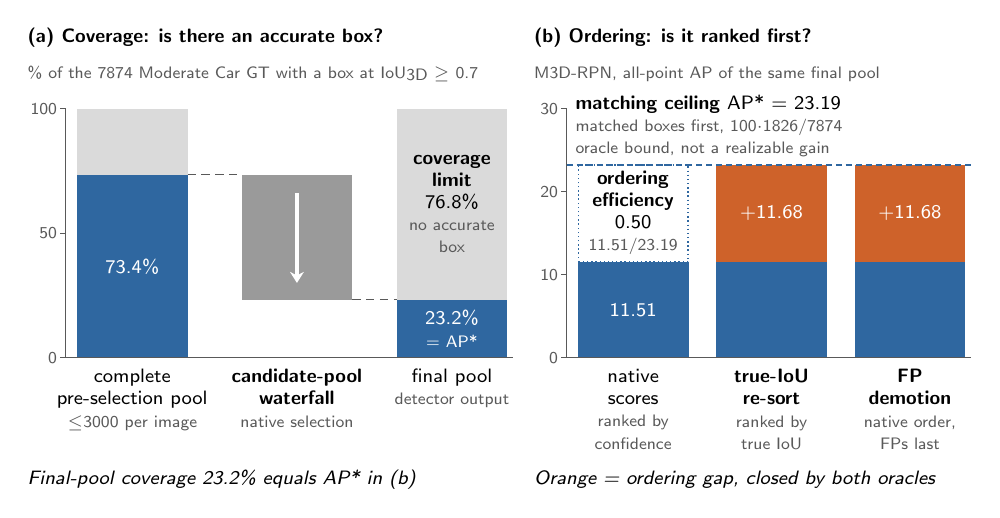
\begin{tikzpicture}[x=1pt,y=1pt,
  title/.style={anchor=base west,font=\fsT\bfseries,inner sep=0},
  unit/.style={anchor=base west,font=\fsD,text=furn,inner sep=0},
  tick/.style={anchor=east,font=\fsD,text=furn,inner sep=1pt},
  cat/.style={anchor=north,align=center,font=\fsL,inner sep=0},
  qty/.style={align=center,font=\fsL,inner sep=0},
  val/.style={font=\fsL,text=white,inner sep=0},
  take/.style={anchor=base west,font=\fsL\itshape,inner sep=0},
  axis/.style={furn,line width=0.4pt},
  conn/.style={furn,line width=0.4pt,densely dashed},
  ceil/.style={acc,line width=0.7pt,dash pattern=on 2.2pt off 1.4pt}]
\def\H{90}
\def\bw{20}   % half bar width
\def\ya{0.9} % (a) pt per percent
\def\yb{3.0} % (b) pt per AP point
% ============ (a) coverage ============
\def\ax{14}
\def\ca{38}\def\cb{97.5}\def\cc{153.5}
\node[title] at (0,\H+24) {(a) Coverage: is there an accurate box?};
\node[unit] at (0,\H+11) {\% of the 7874 Moderate Car GT with a box at \iou\ $\geq$ 0.7};
\draw[axis] (\ax,0) -- (\ax,\H);
\foreach \t in {0,50,100} {\draw[axis] (\ax-2,\t*\ya) -- (\ax,\t*\ya); \node[tick] at (\ax-2,\t*\ya) {\t};}
% complete pool
\fill[acc]  (\ca-\bw,0) rectangle (\ca+\bw,73.4*\ya);
\fill[miss] (\ca-\bw,73.4*\ya) rectangle (\ca+\bw,100*\ya);
\node[val] at (\ca,36.7*\ya) {73.4\%};
% waterfall drop
\fill[drop] (\cb-\bw,23.2*\ya) rectangle (\cb+\bw,73.4*\ya);
\draw[white,line width=1.2pt,-{Stealth[length=4pt,width=5pt]}] (\cb,66*\ya) -- (\cb,30*\ya);
\draw[conn] (\ca+\bw,73.4*\ya) -- (\cb-\bw,73.4*\ya);
\draw[conn] (\cb+\bw,23.2*\ya) -- (\cc-\bw,23.2*\ya);
% final pool
\fill[acc]  (\cc-\bw,0) rectangle (\cc+\bw,23.2*\ya);
\fill[miss] (\cc-\bw,23.2*\ya) rectangle (\cc+\bw,100*\ya);
\node[val,align=center] at (\cc,11.6*\ya) {23.2\%\\{\fsD = AP*}};
\node[qty] at (\cc,61.6*\ya) {\textbf{coverage}\\\textbf{limit}\\76.8\%\\\sub{no accurate}\\\sub{box}};
\draw[axis] (\ax,0) -- (\cc+\bw+2,0);
\node[cat] at (\ca,-4) {complete\\pre-selection pool\\\sub{$\leq$3000 per image}};
\node[cat] at (\cb,-4) {\textbf{candidate-pool}\\\textbf{waterfall}\\\sub{native selection}};
\node[cat] at (\cc,-4) {final pool\\\sub{detector output}};
\node[take] at (0,-46) {Final-pool coverage 23.2\% equals AP* in (b)};
% ============ (b) ordering ============
\begin{scope}[xshift=183pt]
\def\ax{12}
\def\ca{36}\def\cb{86}\def\cc{136}
\node[title] at (0,\H+24) {(b) Ordering: is it ranked first?};
\node[unit] at (0,\H+11) {M3D-RPN, all-point AP of the same final pool};
\draw[axis] (\ax,0) -- (\ax,\H);
\foreach \t in {0,10,20,30} {\draw[axis] (\ax-2,\t*\yb) -- (\ax,\t*\yb); \node[tick] at (\ax-2,\t*\yb) {\t};}
% native
\fill[acc] (\ca-\bw,0) rectangle (\ca+\bw,11.51*\yb);
\node[val] at (\ca,5.75*\yb) {11.51};
\draw[acc,line width=0.5pt,densely dotted] (\ca-\bw+0.25,11.51*\yb) rectangle (\ca+\bw-0.25,23.19*\yb);
\node[qty] at (\ca,17.35*\yb+0.3) {\textbf{ordering}\\\textbf{efficiency}\\0.50\\\sub{11.51/23.19}};
% re-sort and FP demotion
\foreach \c in {\cb,\cc} {
  \fill[acc]  (\c-\bw,0) rectangle (\c+\bw,11.51*\yb);
  \fill[gapc] (\c-\bw,11.51*\yb) rectangle (\c+\bw,23.19*\yb);
  \node[val] at (\c,17.35*\yb) {+11.68};
}
\draw[ceil] (\ax,23.19*\yb) -- (\cc+\bw+2,23.19*\yb);
\node[anchor=south west,align=left,inner sep=0,font=\fsL] at (\ax+3,23.19*\yb+2.8) {\textbf{matching ceiling} AP* = 23.19\\\sub{matched boxes first, 100$\cdot$1826/7874}\\\sub{oracle bound, not a realizable gain}};
\draw[axis] (\ax,0) -- (\cc+\bw+2,0);
\node[cat] at (\ca,-4) {native\\scores\\\sub{ranked by}\\\sub{confidence}};
\node[cat] at (\cb,-4) {\textbf{true-IoU}\\\textbf{re-sort}\\\sub{ranked by}\\\sub{true IoU}};
\node[cat] at (\cc,-4) {\textbf{FP}\\\textbf{demotion}\\\sub{native order,}\\\sub{FPs last}};
\node[take] at (0,-46) {Orange = ordering gap, closed by both oracles};
\end{scope}
\end{tikzpicture}
\end{document}
